% ── Chương 5: RankBoost ──────────────────────────────────────────────────────
\subsection{RankBoost}
\label{sec:rankboost}

RankBoost \citep{freund2003efficient} là một thuật toán boosting cho ranking,
tương tự AdaBoost cho phân loại nhị phân. Ý tưởng cơ bản: kết hợp nhiều
\textit{base ranker} yếu thành một ranker mạnh bằng cách tối ưu hóa trọng số phân phối cặp dữ liệu một cách thích ứng.

\subsubsection{Định nghĩa các đại lượng và Ký hiệu học thuật}

Đặt $\Hcal$ là tập các \textit{base rankers} -- các hàm từ $\Xcal$ vào $\{0, 1\}$ (hoặc tổng quát hơn, vào $[0, 1]$ hay $\R$).

Để mô tả trọng số của phân phối cặp dữ liệu $D_t$ trên tập mẫu huấn luyện, với mỗi vòng $t$ và mỗi trạng thái $s \in \{-1, 0, +1\}$, giáo trình gốc \citep{mohri2018foundations} định nghĩa các biến trọng số tích lũy $\epsilon^s_t$ như sau:
\begin{equation}
    \epsilon^s_t = \sum_{i=1}^m D_t(i) \mathbf{1}_{y_i(h_t(x'_i) - h_t(x_i)) = s}
    = \E_{i \sim D_t}\bigl[\mathbf{1}_{y_i(h_t(x'_i) - h_t(x_i)) = s}\bigr].
    \label{eq:epsilon_def}
\end{equation}
Chúng tôi ký hiệu rút gọn $\epsilon^+_t \equiv \epsilon^{+1}_t$ (tỷ lệ trọng số xếp đúng), $\epsilon^-_t \equiv \epsilon^{-1}_t$ (tỷ lệ trọng số xếp sai), và $\epsilon^0_t \equiv \epsilon^0_t$ (tỷ lệ trọng số không phân biệt được). Hiển nhiên ta luôn có: $\epsilon^+_t + \epsilon^-_t + \epsilon^0_t = 1$.

Để tránh sự lẫn lộn học thuật, chúng tôi tuân thủ nghiêm ngặt ký hiệu của giáo trình Mohri:
\begin{itemize}
    \item Các ký hiệu $\epsilon^+_t, \epsilon^-_t, \epsilon^0_t$ đại diện cho trọng số phân phối biên của các cặp dữ liệu.
    \item Ký hiệu $\gamma_t$ được dành riêng để định nghĩa \textbf{edge} (độ lợi hay biên danh nghĩa) của base ranker $h_t$ tại vòng $t$:
    \begin{equation}
        \gamma_t = \frac{\epsilon^+_t - \epsilon^-_t}{2}.
        \label{eq:edge_def}
    \end{equation}
\end{itemize}

\begin{example}[Tính toán nhanh các đại lượng mẫu biên và Edge]
Giả sử tại một vòng lặp $t$, ta có tập dữ liệu gồm $5$ cặp preference huấn luyện có cùng trọng số phân phối đều: $D_t(i) = 0.2$ với mọi $i \in [5]$. Xét một base ranker yếu $h_t$ cho kết quả so sánh trên $5$ cặp này như sau:
\begin{itemize}
    \item Xếp hạng đúng trên 3 cặp: $y_i(h_t(x'_i) - h_t(x_i)) = +1$ (với $i \in \{1, 3, 4\}$).
    \item Xếp hạng sai trên 1 cặp: $y_i(h_t(x'_i) - h_t(x_i)) = -1$ (với $i = 2$).
    \item Không phân biệt được trên 1 cặp: $y_i(h_t(x'_i) - h_t(x_i)) = 0$ (với $i = 5$).
\end{itemize}
Áp dụng định nghĩa từ công thức \eqref{eq:epsilon_def}, ta có các biến trọng số tích lũy:
\begin{itemize}
    \item $\epsilon^+_t = 0.2 + 0.2 + 0.2 = 0.6$ (tổng trọng số cặp đúng).
    \item $\epsilon^-_t = 0.2$ (tổng trọng số cặp sai).
    \item $\epsilon^0_t = 0.2$ (tổng trọng số cặp không phân biệt).
\end{itemize}
Hiệu số trọng số xếp đúng và xếp sai là $\epsilon^+_t - \epsilon^-_t = 0.4$. Biên danh nghĩa (edge) của base ranker $h_t$ thu được:
\[
    \gamma_t = \frac{\epsilon^+_t - \epsilon^-_t}{2} = \frac{0.6 - 0.2}{2} = 0.2 > 0.
\]
Nếu cận lề tối thiểu của bài toán là $\gamma = 0.1$, ta luôn có $\gamma_t \ge \gamma > 0$, thỏa mãn hoàn hảo \textbf{Weak Ranking Assumption} (Học tốt hơn ngẫu nhiên). Ví dụ này mô tả trực quan các biến trọng số biên được sử dụng xuyên suốt thuật toán.
\end{example}

\begin{figure}[H]
    \centering
    \begin{tikzpicture}[scale=1.0]
        % Draw Axis line
        \draw[thick, ->] (-0.5,0) -- (6.5,0) node[right, font=\small] {Phân phối biên / Biên};
        % Draw tick marks
        \draw (0,0.1) -- (0,-0.1) node[below, font=\tiny] {$0$};
        \draw (3,0.1) -- (3,-0.1) node[below, font=\tiny] {$0.5$};
        \draw (6,0.1) -- (6,-0.1) node[below, font=\tiny] {$1.0$};
        
        % Draw Epsilon points
        \fill[red] (1.2,0) circle (2.5pt) node[above=4pt, font=\small] {$\epsilon^-_t = 0.2$};
        \fill[blue] (4.8,0) circle (2.5pt) node[above=4pt, font=\small] {$\epsilon^+_t = 0.6$};
        
        % Draw arrows and Edge
        \draw[<->, >=stealth, thick, orange!80!black] (1.2,-0.8) -- (4.8,-0.8) node[midway, fill=white, font=\small] {$\epsilon^+_t - \epsilon^-_t = 0.4$};
        \draw[<->, >=stealth, ultra thick, green!50!black] (3,-1.5) -- (4.8,-1.5) node[midway, fill=white, font=\small] {$\gamma_t = \frac{\epsilon^+_t - \epsilon^-_t}{2} = 0.2$};
        
        % Weak ranking minimum edge reference
        \draw[dashed, gray] (3,-2.2) -- (4.2,-2.2) node[midway, below, font=\small] {$\gamma = 0.1$ (Cận lề tối thiểu)};
        \draw (3,-2.1) -- (3,-2.3);
        \draw (4.2,-2.1) -- (4.2,-2.3);
        \node[right, green!50!black, font=\small] at (4.6,-2.2) {$\implies \gamma_t \geq \gamma > 0$};
    \end{tikzpicture}
    \caption{Trực quan hóa lề cặp (nominal edge) $\gamma_t$ và Giả thuyết Weak Ranking trong RankBoost. Để thuật toán hội tụ theo hàm mũ, lề danh nghĩa $\gamma_t$ của base ranker ở mỗi vòng phải lớn hơn một ngưỡng lề tối thiểu $\gamma > 0$.}
    \label{fig:weak_ranking_edge}
\end{figure}

\subsubsection{Pseudocode RankBoost}

Luồng hoạt động thích ứng của RankBoost được trực quan hóa qua sơ đồ khối dưới đây:

\begin{figure}[H]
    \centering
    \begin{tikzpicture}[
        node distance=1.1cm and 1.5cm,
        box/.style={draw, rectangle, rounded corners, fill=blue!5, minimum width=3cm, minimum height=0.8cm, align=center, font=\small},
        proc/.style={draw, rectangle, fill=orange!5, minimum width=3.5cm, minimum height=0.8cm, align=center, font=\small},
        decision/.style={draw, diamond, aspect=2, fill=yellow!5, minimum width=2.5cm, align=center, inner sep=0pt, font=\small},
        arrow/.style={-latex, thick}
    ]
        \node[box] (start) {\textbf{Khởi tạo} \\ $D_1(i) = 1/m$};
        \node[proc, below=of start] (weak) {\textbf{Vòng $t$: Chọn $h_t$} \\ cực tiểu hoá $\epsilon^-_t - \epsilon^+_t$};
        \node[proc, below=of weak] (alpha) {\textbf{Tính trọng số $\alpha_t$} \\ $\alpha_t = \frac{1}{2}\log(\epsilon^+_t / \epsilon^-_t)$};
        \node[proc, below=of alpha] (dist) {\textbf{Cập nhật phân phối $D_{t+1}$} \\ Nhân $e^{-\alpha_t y_i \Delta h_t}$ và chuẩn hoá};
        \node[decision, below=of dist] (loop) {Đạt $T$ vòng?};
        \node[box, right=of loop] (end) {\textbf{Kết quả} \\ $f = \sum_{t=1}^T \alpha_t h_t$};
        
        \draw[arrow] (start) -- (weak);
        \draw[arrow] (weak) -- (alpha);
        \draw[arrow] (alpha) -- (dist);
        \draw[arrow] (dist) -- (loop);
        \draw[arrow] (loop) -- node[above, font=\small] {Có} (end);
        \draw[arrow] (loop.west) -- ++(-1.2,0) |- node[left, pos=0.25, font=\small] {Chưa} (weak.west);
    \end{tikzpicture}
    \caption{Sơ đồ hoạt động của thuật toán RankBoost. Trọng số của phân phối $D_t$ tự động tập trung vào các cặp bị xếp hạng sai qua từng vòng lặp.}
    \label{fig:rankboost_flowchart}
\end{figure}

Chi tiết các bước thực thi được trình bày cụ thể trong Thuật toán~\ref{alg:rankboost}.

\begin{algorithm}[H]
\caption{RankBoost}
\label{alg:rankboost}
\begin{algorithmic}[1]
\REQUIRE Mẫu huấn luyện $S = \{(x_i, x'_i, y_i)\}_{i=1}^m$ với $y_i \in \{-1, +1\}$
\STATE Khởi tạo $D_1(i) = 1/m$ với mọi $i \in [m]$
\FOR{$t = 1$ to $T$}
    \STATE Chọn base ranker $h_t \leftarrow \displaystyle\arg\min_{h \in \Hcal} \left( \epsilon^-_t(h) - \epsilon^+_t(h) \right) \equiv \displaystyle\arg\min_{h \in \Hcal} \E_{i \sim D_t}\bigl[\mathbf{1}_{y_i(h(x'_i)-h(x_i)) = -1} - \mathbf{1}_{y_i(h(x'_i)-h(x_i)) = +1}\bigr]$
    \STATE Tính hệ số tin cậy: $\alpha_t \leftarrow \frac{1}{2}\log\dfrac{\epsilon^+_t}{\epsilon^-_t}$
    \STATE Tính hằng số chuẩn hoá: $Z_t \leftarrow \epsilon^0_t + 2\sqrt{\epsilon^+_t \epsilon^-_t}$
    \STATE Cập nhật phân phối cặp: $D_{t+1}(i) \leftarrow \dfrac{D_t(i) \exp\bigl(-\alpha_t y_i(h_t(x'_i)-h_t(x_i))\bigr)}{Z_t}$
\ENDFOR
\RETURN Bộ phân hạng ensemble mạnh: $f = \sum_{t=1}^T \alpha_t h_t$
\end{algorithmic}
\end{algorithm}

\subsubsection{Trực giác hoạt động của thuật toán}

\begin{itemize}
    \item \textbf{Bước 3} lựa chọn base ranker yếu $h_t$ tốt nhất theo phân phối hiện tại $D_t$, tương đương việc tìm kiếm ranker tối đa hóa edge $\gamma_t$ (hiệu giữa tỷ lệ đúng và tỷ lệ sai).
    \item \textbf{Bước 4}: hệ số tin cậy $\alpha_t > 0$ khi $\epsilon^+_t > \epsilon^-_t$ (đảm bảo giả thiết \textit{weak ranking} tốt hơn ngẫu nhiên). Mô hình yếu càng chính xác thì trọng số đóng góp của nó vào ensemble càng lớn.
    \item \textbf{Bước 5}: $Z_t$ đóng vai trò chuẩn hoá để phân phối $D_{t+1}$ luôn là một phân phối xác suất hợp lệ (tổng bằng 1).
    \item \textbf{Bước 6}: tăng trọng số của những cặp preference bị xếp hạng \textit{sai} (nhân với hệ số $e^{\alpha_t} > 1$) và giảm trọng số các cặp xếp \textit{đúng} (nhân với $e^{-\alpha_t} < 1$). Nhờ đó, vòng lặp kế tiếp buộc thuật toán phải tập trung học các cặp dữ liệu ``khó''.
\end{itemize}

\subsubsection{Đẳng thức toán học nền tảng}

Phân phối thích ứng $D_{t+1}$ tại vòng $t$ có thể biểu diễn tường minh qua bộ phân hạng tích lũy $f_t = \sum_{s=1}^t \alpha_s h_s$ và các tích hệ số chuẩn hóa:
\begin{equation}
    D_{t+1}(i) = \frac{\exp\bigl(-y_i(f_t(x'_i) - f_t(x_i))\bigr)}{m \prod_{s=1}^t Z_s}.
    \label{eq:D_t1_identity}
\end{equation}

\begin{proof}
Chứng minh bằng phương pháp quy nạp toán học.
\begin{itemize}
    \item Với $t = 0$: $D_1(i) = 1/m = e^0/(m \cdot 1)$ (thỏa mãn đẳng thức).
    \item Giả sử đẳng thức đúng cho vòng $t-1$:
    \[
        D_t(i) = \frac{e^{-y_i(f_{t-1}(x'_i) - f_{t-1}(x_i))}}{m \prod_{s=1}^{t-1} Z_s}.
    \]
    \item Xét bước quy nạp tại vòng $t$, thế công thức cập nhật phân phối ở Bước 6:
    \begin{align*}
        D_{t+1}(i)
        &= \frac{D_t(i) \exp(-\alpha_t y_i(h_t(x'_i) - h_t(x_i)))}{Z_t} \\
        &= \frac{e^{-y_i(f_{t-1}(x'_i) - f_{t-1}(x_i))}}{m \prod_{s=1}^{t-1} Z_s} \cdot \frac{e^{-\alpha_t y_i(h_t(x'_i) - h_t(x_i))}}{Z_t} \\
        &= \frac{\exp\bigl(-y_i \left[ \sum_{s=1}^{t-1} \alpha_s (h_s(x'_i) - h_s(x_i)) + \alpha_t (h_t(x'_i) - h_t(x_i)) \right]\bigr)}{m \prod_{s=1}^t Z_s} \\
        &= \frac{\exp\bigl(-y_i(f_t(x'_i) - f_t(x_i))\bigr)}{m \prod_{s=1}^t Z_s}.
    \end{align*}
\end{itemize}
Đẳng thức được chứng minh hoàn chỉnh.
\end{proof}

\subsubsection{Cận trên sai số thực nghiệm (Empirical Error Bound)}

Định lý dưới đây chỉ ra rằng sai số thực nghiệm của RankBoost được đảm bảo giảm nhanh chóng theo hàm mũ khi tăng số vòng boosting.

\begin{figure}[H]
    \centering
    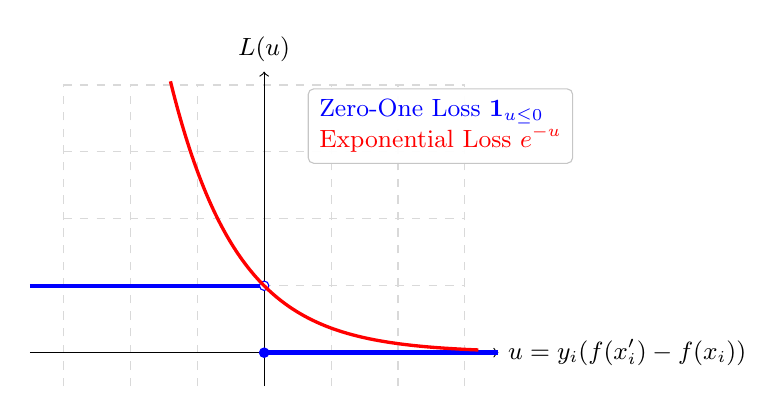
\begin{tikzpicture}[scale=0.85]
        % 1. Draw Grid in background
        \draw[dashed, gray!30] (-3,-0.5) grid (3,4);
        
        % 2. Draw Axes
        \draw[->] (-3.5,0) -- (3.5,0) node[right, font=\small] {$u = y_i(f(x'_i) - f(x_i))$};
        \draw[->] (0,-0.5) -- (0,4.2) node[above, font=\small] {$L(u)$};
        
        % 3. Draw Zero-One Loss (Blue)
        \draw[blue, ultra thick] (-3.5,1) -- (0,1);
        \draw[blue, ultra thick] (0,0) -- (3.5,0);
        \draw[blue, fill=white] (0,1) circle (2pt);
        \draw[blue, fill=blue] (0,0) circle (2pt);
        
        % 4. Draw Exponential Loss (Red)
        \draw[red, very thick, smooth, samples=100, domain=-1.4:3.2] plot (\x, {exp(-\x)});
        
        % 5. Legend kept away from curves/axes to avoid text overlap
        \node[
            draw=gray!45,
            rounded corners=2pt,
            fill=white,
            fill opacity=0.95,
            text opacity=1,
            anchor=north west,
            align=left,
            inner sep=4pt,
            font=\small
        ] at (0.65,3.95) {
            \textcolor{blue}{Zero-One Loss $\mathbf{1}_{u \leq 0}$}\\
            \textcolor{red}{Exponential Loss $e^{-u}$}
        };
    \end{tikzpicture}
    \caption{So sánh Zero-One Loss và Exponential Loss (minh họa toán học cho Định lý~\ref{thm:rankboost_error}). Hàm mũ $e^{-u}$ hoạt động như một cận trên lồi chặt (convex upper bound) cho hàm chỉ thị $\mathbf{1}_{u \leq 0}$, giúp tối ưu hóa bằng phương pháp gradient lồi thuận lợi hơn.}
    \label{fig:loss_comparison}
\end{figure}

\begin{theorem}{Empirical Error Bound for RankBoost (Theorem 10.3)}{rankboost_error}
Empirical error của bộ phân hạng mạnh $f$ tạo bởi RankBoost thỏa mãn hệ thức:
\begin{equation}
    \RS(f) \leq \exp\Biggl(-2 \sum_{t=1}^T \biggl(\frac{\epsilon^+_t - \epsilon^-_t}{2}\biggr)^2\Biggr) = \exp\Biggl(-2 \sum_{t=1}^T \gamma_t^2\Biggr).
    \label{eq:rankboost_bound}
\end{equation}
Hơn thế nữa, nếu thỏa mãn giả thiết \textbf{Weak Ranking Assumption}: tồn tại biên tối thiểu $\gamma > 0$ sao cho với mọi $t \in [T]$, $\gamma_t = \frac{\epsilon^+_t - \epsilon^-_t}{2} \geq \gamma$, thì sai số giảm theo hàm mũ:
\begin{equation}
    \RS(f) \leq \exp(-2\gamma^2 T).
    \label{eq:rankboost_exp_bound}
\end{equation}
\end{theorem}

\begin{proof}[Chứng minh chi tiết]
\textbf{Bước 1: Sử dụng bất đẳng thức lồi chặn trên $\mathbf{1}_{u \leq 0} \leq e^{-u}$ (xem Hình~\ref{fig:loss_comparison}).}

Đặt biến lề cặp $u_i = y_i(f(x'_i) - f(x_i))$. Sai số phân hạng thực nghiệm được định nghĩa:
\begin{align*}
    \RS(f) &= \frac{1}{m} \sum_{i=1}^m \mathbf{1}_{y_i(f(x'_i) - f(x_i)) \leq 0} \\
    &\leq \frac{1}{m} \sum_{i=1}^m \exp\bigl(-y_i(f(x'_i) - f(x_i))\bigr) \\
    &\stackrel{\eqref{eq:D_t1_identity}}{=} \frac{1}{m} \sum_{i=1}^m \left( m \cdot D_{T+1}(i) \prod_{t=1}^T Z_t \right) \\
    &= \left( \prod_{t=1}^T Z_t \right) \cdot \underbrace{\sum_{i=1}^m D_{T+1}(i)}_{=1} = \prod_{t=1}^T Z_t.
\end{align*}

\textbf{Bước 2: Phân tích và tính hằng số chuẩn hoá $Z_t$.}

Theo định nghĩa của $Z_t$:
\begin{align*}
    Z_t &= \sum_{i=1}^m D_t(i) \exp\bigl(-\alpha_t y_i(h_t(x'_i) - h_t(x_i))\bigr) \\
    &= \epsilon^+_t e^{-\alpha_t} + \epsilon^-_t e^{\alpha_t} + \epsilon^0_t.
\end{align*}
Thế hệ số tin cậy tối ưu $\alpha_t = \frac{1}{2}\log(\epsilon^+_t/\epsilon^-_t)$, ta có:
\begin{align*}
    Z_t &= \epsilon^+_t \sqrt{\frac{\epsilon^-_t}{\epsilon^+_t}} + \epsilon^-_t \sqrt{\frac{\epsilon^+_t}{\epsilon^-_t}} + \epsilon^0_t \\
    &= 2\sqrt{\epsilon^+_t \epsilon^-_t} + \epsilon^0_t.
\end{align*}

\textbf{Bước 3: Tìm cận trên cho hệ số chuẩn hoá $Z_t$.}

Vì $\epsilon^+_t + \epsilon^-_t + \epsilon^0_t = 1$, ta biến đổi số hạng dưới dấu căn:
\[
    4\epsilon^+_t \epsilon^-_t = (\epsilon^+_t + \epsilon^-_t)^2 - (\epsilon^+_t - \epsilon^-_t)^2
    = (1 - \epsilon^0_t)^2 - (\epsilon^+_t - \epsilon^-_t)^2.
\]
Thay vào biểu thức $Z_t$:
\begin{align*}
    Z_t &= \sqrt{(1 - \epsilon^0_t)^2 - (\epsilon^+_t - \epsilon^-_t)^2} + \epsilon^0_t \\
    &= (1 - \epsilon^0_t)\sqrt{1 - \frac{(\epsilon^+_t - \epsilon^-_t)^2}{(1 - \epsilon^0_t)^2}} + \epsilon^0_t \\
    &\stackrel{(*)}{\leq} (1 - \epsilon^0_t)\biggl(1 - \frac{(\epsilon^+_t - \epsilon^-_t)^2}{2(1 - \epsilon^0_t)^2}\biggr) + \epsilon^0_t \\
    &= 1 - \frac{(\epsilon^+_t - \epsilon^-_t)^2}{2(1 - \epsilon^0_t)} \\
    &\stackrel{(**)}{\leq} \exp\biggl(-\frac{(\epsilon^+_t - \epsilon^-_t)^2}{2(1 - \epsilon^0_t)}\biggr) \\
    &\leq \exp\biggl(-\frac{(\epsilon^+_t - \epsilon^-_t)^2}{2}\biggr) \quad (\text{do } 1 - \epsilon^0_t \leq 1) \\
    &= \exp\bigl(-2[(\epsilon^+_t - \epsilon^-_t)/2]^2\bigr) = \exp(-2\gamma_t^2).
\end{align*}
Trong đó:
\begin{itemize}
    \item (*): Áp dụng tính lõm của hàm căn thức $\sqrt{1 - x} \leq 1 - x/2$ với mọi $x \le 1$.
    \item (**): Áp dụng bất đẳng thức cơ bản $1 - x \leq e^{-x}$ với mọi $x \in \R$.
\end{itemize}

\textbf{Bước 4: Tổng hợp tích tích lũy.}

Nhân tích lũy cận của các vòng từ $t = 1$ đến $T$:
\[
    \RS(f) \leq \prod_{t=1}^T Z_t \leq \exp\Biggl(-2 \sum_{t=1}^T \gamma_t^2\Biggr).
\]
Định lý được chứng minh hoàn chỉnh và chặt chẽ.
\end{proof}

\begin{example}[Ứng dụng số cho Cận sai số huấn luyện giảm theo hàm mũ]
Để minh họa ý nghĩa thực tiễn của Định lý \ref{thm:rankboost_error}, giả sử chúng ta chạy RankBoost trong $T = 3$ vòng lặp. Tại mỗi vòng lặp $t$, base ranker yếu được chọn đạt được biên độ lợi thế (edge) không đổi là $\gamma_t = 0.3$ (tương đương hiệu số tỷ lệ phân bổ trọng số xếp đúng và sai là $\epsilon^+_t - \epsilon^-_t = 0.6$).

Theo công thức cận trên sai số thực nghiệm \eqref{eq:rankboost_bound}, ta có:
\[
    \RS(f) \leq \exp\left( -2 \sum_{t=1}^3 \gamma_t^2 \right) = \exp\left( -2 \times (0.3^2 + 0.3^2 + 0.3^2) \right) = \exp(-2 \times 0.27) = \exp(-0.54) \approx 0.5827
\]
Như vậy, chỉ sau 3 vòng lặp với một base ranker rất yếu (chỉ tốt hơn ngẫu nhiên một chút), cận trên của tỷ lệ cặp bị xếp hạng sai trên tập huấn luyện đã được đảm bảo giảm xuống còn dưới $58.27\%$. 

Nếu chúng ta tiếp tục chạy đến $T = 10$ vòng lặp với cùng biên độ $\gamma_t = 0.3$, sai số thực nghiệm được đảm bảo:
\[
    \RS(f) \leq \exp(-2 \times 10 \times 0.09) = \exp(-1.8) \approx 0.1653 \quad (\text{dưới } 16.53\%).
\]
Và nếu chạy tới $T = 25$ vòng lặp:
\[
    \RS(f) \leq \exp(-2 \times 25 \times 0.09) = \exp(-4.5) \approx 0.0111 \quad (\text{dưới } 1.11\%).
\]
Điều này cho thấy trực quan tốc độ hội tụ cực nhanh theo hàm mũ của RankBoost, ngay cả khi các base ranker được chọn ở mỗi vòng chỉ có độ lợi thế vô cùng nhỏ bé. Tốc độ suy giảm sai số huấn luyện này được biểu diễn trực quan qua Hình \ref{fig:exponential_error_decay}.
\end{example}

\begin{figure}[H]
    \centering
    \begin{tikzpicture}
        \begin{axis}[
            xlabel={Số vòng lặp $T$},
            ylabel={Cận trên sai số $\exp(-2\gamma^2 T)$},
            xmin=0, xmax=30,
            ymin=0, ymax=1,
            xtick={0,5,10,15,20,25,30},
            ytick={0,1},
            grid=both,
            grid style={dashed, gray!30},
            legend style={at={(0.7,0.8)}, anchor=west, font=\tiny},
            width=10.5cm,
            height=6.2cm
        ]
            % Plot for gamma = 0.1 -> exp(-x/50)
            \addplot[blue, thick, domain=0:30, samples=100] {exp(-x/50)};
            \addlegendentry{$\gamma = 0.1$};
            
            % Plot for gamma = 0.2 -> exp(-2*x/25)
            \addplot[orange, thick, domain=0:30, samples=100] {exp(-2*x/25)};
            \addlegendentry{$\gamma = 0.2$};
            
            % Plot for gamma = 0.3 -> exp(-9*x/50)
            \addplot[red, ultra thick, domain=0:30, samples=100] {exp(-9*x/50)};
            \addlegendentry{$\gamma = 0.3$};
        \end{axis}
    \end{tikzpicture}
    \caption{Tốc độ suy giảm theo hàm mũ của cận trên sai số thực nghiệm RankBoost ứng với các giá trị biên danh nghĩa $\gamma$ khác nhau. Biên độ $\gamma$ càng lớn (base ranker càng mạnh), sai số huấn luyện hội tụ về $0$ càng nhanh.}
    \label{fig:exponential_error_decay}
\end{figure}

\begin{tcolorbox}[enhanced, breakable, colback=blue!5, colframe=blue!50!black, title={\textbf{Cận hội tụ dưới điều kiện yếu hơn (Weaker Edge Condition)}}]
Trong trường hợp tổng quát hơn, giáo trình Mohri (trang 248) chỉ ra rằng một điều kiện yếu hơn cũng đủ để RankBoost hội tụ theo hàm mũ. Cụ thể, nếu tồn tại $\gamma > 0$ sao cho với mọi $t \in [T]$:
\begin{equation}
    \gamma_t \geq \gamma \sqrt{1 - \epsilon^0_t} \quad \Longleftrightarrow \quad \gamma \leq \frac{\epsilon^+_t - \epsilon^-_t}{2\sqrt{1 - \epsilon^0_t}},
    \label{eq:weaker_edge}
\end{equation}
thì hằng số chuẩn hóa $Z_t \leq \exp(-2\gamma^2)$ vẫn được đảm bảo, dẫn đến sai số huấn luyện giảm nhanh theo hàm mũ $\RS(f) \leq \exp(-2\gamma^2 T)$. Điều này cho thấy thuật toán hoạt động cực kỳ linh hoạt ngay cả khi phần lớn các cặp dữ liệu không phân biệt được ($\epsilon^0_t$ lớn).
\end{tcolorbox}

\subsubsection{Ví dụ tính toán từng bước minh hoạ RankBoost}

Giả sử chúng ta có 3 đối tượng $\{a, b, c\}$ với thứ tự thực tế là $c > b > a$. Tập dữ liệu huấn luyện gồm 3 cặp preference có nhãn $y_i = +1$:
\begin{enumerate}
    \item $p_1 = (c, b)$ với nhãn $y_1 = +1$ (c cao hơn b)
    \item $p_2 = (b, a)$ với nhãn $y_2 = +1$ (b cao hơn a)
    \item $p_3 = (c, a)$ với nhãn $y_3 = +1$ (c cao hơn a)
\end{enumerate}
Giả sử tại vòng $t = 1$, phân phối trọng số ban đầu không đều: $D_1 = [0.5, 0.2, 0.3]$.

Xét một base ranker $h_1$ được chọn thỏa mãn:
\begin{itemize}
    \item Xếp đúng cặp $p_1$: $h_1(c) - h_1(b) = 1 \implies y_1 \cdot \text{diff} = 1$
    \item Xếp sai cặp $p_2$: $h_1(b) - h_1(a) = -1 \implies y_2 \cdot \text{diff} = -1$
    \item Xếp đúng cặp $p_3$: $h_1(c) - h_1(a) = 1 \implies y_3 \cdot \text{diff} = 1$
\end{itemize}

Tính toán trọng số tích lũy trên phân phối $D_1$:
\begin{itemize}
    \item $\epsilon^+_1 = D_1(1) + D_1(3) = 0.5 + 0.3 = 0.8$ (tổng trọng số xếp đúng)
    \item $\epsilon^-_1 = D_1(2) = 0.2$ (tổng trọng số xếp sai)
    \item $\epsilon^0_1 = 0.0$ (không có cặp phân biệt trùng)
\end{itemize}
Biên của base ranker đạt: $\gamma_1 = (\epsilon^+_1 - \epsilon^-_1)/2 = 0.3$.

Hệ số tin cậy đóng góp của base ranker $h_1$ là:
\[
    \alpha_1 = \frac{1}{2} \log\left(\frac{\epsilon^+_1}{\epsilon^-_1}\right) = \frac{1}{2} \log\left(\frac{0.8}{0.2}\right) = \log(2) \approx 0.693
\]
Hằng số chuẩn hoá $Z_1$ là:
\[
    Z_1 = 2\sqrt{\epsilon^+_1 \epsilon^-_1} + \epsilon^0_1 = 2\sqrt{0.8 \times 0.2} + 0 = 0.8
\]

Cập nhật phân phối $D_2$ thích ứng cho vòng sau:
\begin{itemize}
    \item Cặp xếp đúng $p_1$: $D_2(1) = \frac{D_1(1) e^{-\alpha_1}}{Z_1} = \frac{0.5 \times 0.5}{0.8} = 0.3125$
    \item Cặp xếp sai $p_2$: $D_2(2) = \frac{D_1(2) e^{\alpha_1}}{Z_1} = \frac{0.2 \times 2}{0.8} = 0.5000$
    \item Cặp xếp đúng $p_3$: $D_2(3) = \frac{D_1(3) e^{-\alpha_1}}{Z_1} = \frac{0.3 \times 0.5}{0.8} = 0.1875$
\end{itemize}

\begin{figure}[H]
    \centering
    \begin{tikzpicture}[scale=0.85]
        \begin{axis}[
            ybar,
            enlargelimits=0.15,
            legend style={at={(0.5,-0.2)}, anchor=north, legend columns=-1},
            ylabel={Trọng số phân phối $D_t(i)$},
            symbolic x coords={Cặp 1 (Đúng), Cặp 2 (Sai), Cặp 3 (Đúng)},
            xtick=data,
            nodes near coords,
            nodes near coords align={vertical},
            ymin=0, ymax=0.6,
            bar width=18pt,
            width=10.5cm,
            height=6.2cm
        ]
            \addplot[fill=blue!30, draw=blue] coordinates {
                (Cặp 1 (Đúng), 0.5)
                (Cặp 2 (Sai), 0.2)
                (Cặp 3 (Đúng), 0.3)
            };
            \addplot[fill=orange!40, draw=orange] coordinates {
                (Cặp 1 (Đúng), 0.3125)
                (Cặp 2 (Sai), 0.5)
                (Cặp 3 (Đúng), 0.1875)
            };
            \legend{Vòng $t=1$ ($D_1$), Vòng $t=2$ ($D_2$)}
        \end{axis}
    \end{tikzpicture}
    \caption{Sự thay đổi trọng số phân phối cặp $D_t$ qua 2 vòng boosting trong ví dụ huấn luyện (minh họa thực tế cho cơ chế cập nhật của RankBoost). Trọng số của cặp bị xếp sai $p_2$ tăng vọt từ $0.20$ lên $0.50$, ép thuật toán vòng sau phải sửa chữa lỗi sai này.}
    \label{fig:weight_shift}
\end{figure}

Sự phân bổ lại trọng số phân phối được trực quan hóa tại Hình~\ref{fig:weight_shift}. Trọng số của cặp xếp sai tăng vọt làm cơ sở thúc đẩy RankBoost tăng cường độ chính xác liên tục.

\begin{morong}
\textbf{[MỞ RỘNG] Phản ví dụ: Sự sụp đổ của Weak Ranking Assumption với Preference Cycle.}

Một giả thiết tối quan trọng để RankBoost hội tụ là \textit{Weak Ranking Assumption}: tồn tại $\gamma > 0$ sao cho ở mỗi vòng $\gamma_t \geq \gamma > 0$. Chúng ta sẽ xây dựng một ví dụ phản chứng chỉ ra rằng khi preference chứa \textbf{chu trình không bắc cầu} (non-transitive cycles), giả thiết này sẽ bị vi phạm và RankBoost không thể học được hoàn hảo.

Xét 3 phần tử $\{x_1, x_2, x_3\}$ có preference dạng chu trình kéo theo:
\[
    f(x_1, x_2) = +1, \quad f(x_2, x_3) = +1, \quad f(x_3, x_1) = +1.
\]
Giả sử tập giả thuyết $\Hcal$ gồm các scoring functions tuyến tính $h(x) = w \cdot x$. Do scoring function luôn cảm sinh một thứ tự bắc cầu (transitive), các thứ tự có thể biểu diễn bởi $h \in \Hcal$ chỉ có thể là các hoán vị tuyến tính không có chu trình. 

Bất kỳ hoán vị tuyến tính nào trên 3 phần tử cũng chỉ có thể xếp đúng tối đa 2 trong 3 cặp preference trên và bắt buộc phải xếp sai ít nhất 1 cặp.
Giả sử tại vòng $t$, phân phối trọng số hội tụ về dạng đều trên các cặp: $D_t = [1/3, 1/3, 1/3]$. Khi đó, với bất kỳ base ranker $h \in \Hcal$ nào:
\begin{itemize}
    \item Nếu $h$ xếp đúng 2 cặp và xếp sai 1 cặp: $\epsilon^+_t = 2/3$ và $\epsilon^-_t = 1/3 \implies \gamma_t = (\epsilon^+_t - \epsilon^-_t)/2 = 1/6 > 0$.
    \item Tuy nhiên, khi RankBoost tăng trọng số của cặp bị xếp sai lên, phân phối $D$ sẽ thay đổi. Khi phân phối đạt trạng thái cân bằng nơi mà các cặp khó xoay vòng, không còn bất kỳ base ranker nào trong $\Hcal$ có thể đạt được $\epsilon^+_t > \epsilon^-_t$ (chỉ có thể đạt $\epsilon^+_t = \epsilon^-_t$ do tính đối xứng của chu trình).
\end{itemize}
Tại thời điểm đó, $\gamma_t = 0 \implies \alpha_t = 0$. Thuật toán dừng lại và \textbf{không thể giảm empirical error về 0}. Điều này phản ánh hạn chế cấu trúc của score-based setting khi đối mặt với preference cycles của con người.
\end{morong}

\subsubsection{Liên hệ với Coordinate Descent}

\begin{theorem}{RankBoost $\equiv$ Coordinate Descent (Section 10.4.2)}{rb_cd}
RankBoost tương đương với việc áp dụng \textit{coordinate descent} trên hàm mục tiêu lồi:
\begin{equation}
    F(\bm{\alpha}) = \sum_{i=1}^m \exp\Biggl(-y_i \sum_{j=1}^N \alpha_j (h_j(x'_i) - h_j(x_i))\Biggr).
    \label{eq:F_obj}
\end{equation}
\end{theorem}

\begin{proof}[Chứng minh bằng phương pháp quy nạp toán học]
Ta tiến hành chứng minh sự tương đương tuyệt đối giữa hai thuật toán bằng phương pháp quy nạp toán học theo số vòng boosting $t$.

Đặt $f_t = \sum_{s=1}^t \alpha_s h_s$ là bộ phân hạng mạnh tích lũy của thuật toán RankBoost tại vòng $t$, tương ứng với vectơ trọng số $\bm{\alpha}_t \in \R^N$ có các thành phần $\alpha_s$ (với $s \le t$) và các thành phần khác bằng $0$.
Đặt $\bar{f}_t$ là bộ phân hạng của Coordinate Descent tại vòng $t$, tương ứng với vectơ trọng số $\bar{\bm{\alpha}}_t \in \R^N$.

\begin{itemize}
    \item \textbf{Bước cơ sở ($t=0$):} Ở vạch xuất phát, cả hai thuật toán đều khởi tạo vectơ trọng số bằng vectơ không: $\bm{\alpha}_0 = \bar{\bm{\alpha}}_0 = \bm{0} \implies f_0 = \bar{f}_0 \equiv 0$. Do đó, phân phối cặp khởi đầu của cả hai đều là phân phối đều: $D_1 = \bar{D}_1 = [1/m, \dots, 1/m]$. Đẳng thức thỏa mãn.
    
    \item \textbf{Giả thiết quy nạp:} Giả sử đẳng thức đúng cho vòng $t-1$, nghĩa là bộ phân hạng tích lũy của hai thuật toán trùng nhau:
    \[
        \bar{\bm{\alpha}}_{t-1} = \bm{\alpha}_{t-1} \implies \bar{f}_{t-1} = f_{t-1}.
    \]
    Hệ quả trực tiếp là phân phối cặp cảm sinh bởi hai mô hình tại đầu vòng $t$ trùng nhau hoàn toàn: $\bar{D}_t = D_t$.
    
    \item \textbf{Bước quy nạp (Vòng $t$):} Ta chứng minh Coordinate Descent sẽ lựa chọn hướng tọa độ và độ dài bước đi trùng khít với việc chọn base ranker $h_t$ và trọng số $\alpha_t$ của RankBoost.
    
    \textbf{1. Tìm hướng đi tối ưu (Chọn coordinate $e_k$):}
    Tại bước $t$, Coordinate Descent tìm kiếm hướng tọa độ đơn vị $e_k$ (tương ứng với base ranker $h_k \in \mathcal{H}$) để cực tiểu hóa đạo hàm theo hướng (\textit{directional derivative}) của hàm loss mục tiêu $F$ tại điểm $\bm{\alpha}_{t-1}$:
    \[
        F'(\bm{\alpha}_{t-1}; e_k) = \lim_{\eta \to 0} \frac{F(\bm{\alpha}_{t-1} + \eta e_k) - F(\bm{\alpha}_{t-1})}{\eta}.
    \]
    Khai triển đạo hàm riêng theo hướng $\eta$ tại điểm $\eta = 0$:
    \begin{align*}
        F'(\bm{\alpha}_{t-1}; e_k)
        &= -\sum_{i=1}^m y_i (h_k(x'_i) - h_k(x_i)) \exp\Biggl(-y_i \sum_{j=1}^N \alpha_{t-1,j}(h_j(x'_i) - h_j(x_i))\Biggr) \\
        &= -\sum_{i=1}^m y_i (h_k(x'_i) - h_k(x_i)) D_t(i) m \prod_{s=1}^{t-1} Z_s \quad (\text{áp dụng đẳng thức quy nạp } \eqref{eq:D_t1_identity}) \\
        &= -m \left( \prod_{s=1}^{t-1} Z_s \right) \left[ \sum_{i: y_i \Delta h_k = 1} D_t(i) - \sum_{i: y_i \Delta h_k = -1} D_t(i) \right] \\
        &= -m \left( \prod_{s=1}^{t-1} Z_s \right) [\epsilon^+_t - \epsilon^-_t] = -2\gamma_t \cdot m \prod_{s=1}^{t-1} Z_s.
    \end{align*}
    Do hằng số $m \prod_{s=1}^{t-1} Z_s > 0$ cố định tại đầu vòng $t$, việc cực tiểu hóa đạo hàm hướng $F'(\bm{\alpha}_{t-1}; e_k)$ tương đương tuyệt đối với việc \textbf{cực đại hóa độ lợi thế $\gamma_t$} (nominal edge). Đây chính xác là tiêu chí chọn base ranker yếu $h_t$ tốt nhất ở Bước 3 của RankBoost:
    \[
        h_t = \arg\max_{h \in \mathcal{H}} \gamma_t(h) = \arg\min_{h \in \mathcal{H}} (\epsilon^-_t(h) - \epsilon^+_t(h)).
    \]
    Như vậy, Coordinate Descent chọn đúng tọa độ tương ứng với base ranker $h_t$ của RankBoost.
    
    \textbf{2. Tìm bước nhảy tối ưu (Line Search độ dài $\eta$):}
    Sau khi đã xác định hướng tọa độ $e_t$ tương ứng với $h_t$, Coordinate Descent giải bài toán tìm kiếm đường thẳng (exact line search) để tìm độ dài bước nhảy $\eta > 0$ tối ưu:
    \[
        \eta = \arg\min_{\eta} F(\bm{\alpha}_{t-1} + \eta e_t).
    \]
    Lấy đạo hàm của hàm số một biến theo $\eta$ và giải phương trình đạo hàm bằng $0$:
    \begin{align*}
        &\frac{dF(\bm{\alpha}_{t-1} + \eta e_t)}{d\eta} = 0 \\
        &\iff -\sum_{i=1}^m y_i (h_t(x'_i) - h_t(x_i)) \\
        &\qquad \times \exp\Biggl(-y_i \sum_{j=1}^N \alpha_{t-1,j} (h_j(x'_i) - h_j(x_i)) - y_i \eta (h_t(x'_i) - h_t(x_i)) \Biggr) = 0 \\
        &\iff -\sum_{i=1}^m y_i \Delta h_t D_t(i) e^{-\eta y_i \Delta h_t} = 0 \quad (\text{thế phân phối } D_t) \\
        &\iff -\left[ \sum_{i: y_i \Delta h_t = 1} D_t(i) e^{-\eta} - \sum_{i: y_i \Delta h_t = -1} D_t(i) e^{\eta} \right] = 0 \\
        &\iff -\epsilon^+_t e^{-\eta} + \epsilon^-_t e^{\eta} = 0 \\
        &\iff e^{2\eta} = \frac{\epsilon^+_t}{\epsilon^-_t} \iff \eta = \frac{1}{2}\log\frac{\epsilon^+_t}{\epsilon^-_t}.
    \end{align*}
    Giá trị độ dài bước tối ưu $\eta$ này khớp chính xác tuyệt đối với hệ số tin cậy $\alpha_t$ của RankBoost.
    
    \textbf{3. Cập nhật trạng thái:}
    Vectơ trọng số mới của hai thuật toán trùng nhau:
    \[
        \bar{\bm{\alpha}}_t = \bar{\bm{\alpha}}_{t-1} + \eta e_t = \bm{\alpha}_{t-1} + \alpha_t e_t = \bm{\alpha}_t \implies \bar{f}_t = f_t.
    \]
\end{itemize}
Chứng minh quy nạp hoàn tất. RankBoost và Coordinate Descent là đồng nhất về mặt toán học.
\end{proof}

\begin{figure}[H]
    \centering
    \begin{tikzpicture}[scale=0.9]
        % Draw Contour lines of a convex function
        \draw[gray!40, thick] (3,2) ellipse (0.6cm and 0.4cm);
        \draw[gray!40, thick] (3,2) ellipse (1.5cm and 1.0cm);
        \draw[gray!40, thick] (3,2) ellipse (2.5cm and 1.7cm);
        \draw[gray!40, thick] (3,2) ellipse (3.6cm and 2.4cm);
        \draw[gray!40, thick] (3,2) ellipse (4.8cm and 3.2cm);
        
        % Optimum point
        \fill[red] (3,2) circle (2pt) node[above right, font=\tiny] {$\bm{\alpha}^*$ (Tối ưu)};
        
        % Coordinate Axes
        \draw[thick, ->] (-0.5,0) -- (6.0,0) node[right, font=\tiny] {$\alpha_1$ ($h_1$)};
        \draw[thick, ->] (0,-0.5) -- (0,4.5) node[above, font=\tiny] {$\alpha_2$ ($h_2$)};
        
        % Coordinate Descent Trajectory Steps
        \draw[ultra thick, blue, ->, >=stealth] (0,0) -- (1.8,0) node[midway, below=3pt, font=\tiny] {Bước 1 ($\alpha_1$)};
        \draw[ultra thick, blue, ->, >=stealth] (1.8,0) -- (1.8,1.4) node[midway, right=3pt, font=\tiny] {Bước 2 ($\alpha_2$)};
        \draw[ultra thick, blue, ->, >=stealth] (1.8,1.4) -- (2.6,1.4) node[midway, below=2pt, font=\tiny] {Bước 3};
        \draw[ultra thick, blue, ->, >=stealth] (2.6,1.4) -- (2.6,1.85) node[midway, right=2pt, font=\tiny] {Bước 4};
        \draw[ultra thick, blue, ->, >=stealth] (2.6,1.85) -- (2.9,1.85);
        \draw[ultra thick, blue, ->, >=stealth] (2.9,1.85) -- (2.9,1.97) -- (3.0,2.0);
        
        % Start point
        \fill[black] (0,0) circle (2.5pt) node[below left, font=\tiny] {$\bm{\alpha}_0 = \bm{0}$};
    \end{tikzpicture}
    \caption{Trực quan hóa quỹ đạo tối ưu hóa của RankBoost thông qua Coordinate Descent trên không gian 2D của trọng số $\bm{\alpha}$. Thuật toán bắt đầu từ gốc tọa độ $\bm{\alpha}_0 = \bm{0}$ và di chuyển vuông góc dọc theo các trục tọa độ (mỗi trục đại diện cho một base ranker $h_j$) để tiệm cận về điểm cực tiểu toàn cục $\bm{\alpha}^*$.}
    \label{fig:coordinate_descent_steps}
\end{figure}

\begin{tcolorbox}[enhanced, breakable, colback=blue!5, colframe=blue!50!black]
\textbf{Nhận xét}: Phương trình \eqref{eq:F_obj} là một cận trên lồi chặt của hàm tổn thất nhị phân thực tế. RankBoost thực chất chính là giải pháp tối ưu hóa tối tân sử dụng gradient lồi trên bao lồi của các bộ phân hạng yếu.
\end{tcolorbox}

\subsubsection{Margin bound cho ensemble methods trong ranking}

\begin{corollary}{Margin Bound for Ensembles in Ranking (Corollary 10.4)}{ensemble_bound}
Cho $\Hcal$ là tập hàm thực. Với $\rho > 0$, $\delta > 0$, với xác suất ít nhất $1 - \delta$, với mọi bộ phân hạng ensemble lồi $h \in \conv(\Hcal)$:
\begin{equation}
    R(h) \leq \RR{\rho}(h) + \frac{2}{\rho}\bigl[R^{D_1}_m(\Hcal) + R^{D_2}_m(\Hcal)\bigr] + \sqrt{\frac{\log(1/\delta)}{2m}}.
    \label{eq:ensemble_bound_formula}
\end{equation}
Trong đó, $\RR{\rho}(h) \equiv \widehat{R}_{S,\rho}(h)$ là \textbf{empirical margin ranking loss} (sai số lề thực nghiệm trên tập mẫu $S$ với lề $\rho$) và hai số hạng Rademacher $\mathfrak{R}_m^{D_1}(\mathcal{H})$ và $\mathfrak{R}_m^{D_2}(\mathcal{H})$ đều có cùng kích thước mẫu là $m$ vì đây là cận tổng quát (general bound) cho preference ranking của giáo trình Mohri. Tuy nhiên, cần lưu ý một điểm tinh tế rằng khi áp dụng sang bipartite ranking, do các mẫu tích cực và tiêu cực được lấy độc lập từ hai phân phối riêng biệt với kích thước mẫu lần lượt là $m$ và $n$, cận Rademacher tương ứng sẽ tách thành hai số hạng ứng với hai kích thước mẫu khác nhau là $\mathfrak{R}_m^{D^+}(\mathcal{H})$ và $\mathfrak{R}_n^{D^-}(\mathcal{H})$.
\end{corollary}

\begin{proof}[Chứng minh chi tiết]
Ta tiến hành chứng minh hệ thức dựa trên việc áp dụng Định lý tổng quát \ref{thm:margin_ranking} cho không gian giả thuyết mở rộng $\conv(\Hcal)$ kết hợp với bổ đề Rademacher của bao lồi:

\begin{enumerate}
    \item \textbf{Bước 1: Định lý tổng quát về chặn lề phân hạng cho không gian giả thuyết $\conv(\Hcal)$.}
    Áp dụng Định lý tổng quát về chặn lề phân hạng (ở đây là Theorem 10.1 của giáo trình Mohri) cho tập các giả thuyết là bao lồi lồi $\conv(\Hcal)$ thay cho $\Hcal$, ta thu được với xác suất ít nhất $1 - \delta$, với mọi $h \in \conv(\Hcal)$:
    \begin{equation}
        R(h) \leq \RR{\rho}(h) + \frac{2}{\rho}\bigl[R^{D_1}_m(\conv(\Hcal)) + R^{D_2}_m(\conv(\Hcal))\bigr] + \sqrt{\frac{\log(1/\delta)}{2m}}.
        \label{eq:ensemble_step1}
    \end{equation}
    Trong đó, $R^{D_1}_m(\conv(\Hcal))$ và $R^{D_2}_m(\conv(\Hcal))$ lần lượt là Rademacher Complexity tổng quát của bao lồi $\conv(\Hcal)$ trên phân phối biên $D_1$ và $D_2$ với mẫu kích thước $m$.
    
    \item \textbf{Bước 2: Áp dụng Bổ đề 7.4 (Rademacher complexity của bao lồi).}
    Một kết quả lý thuyết kinh điển của Rademacher Complexity chỉ ra rằng độ phức tạp Rademacher thực nghiệm của bao lồi $\conv(\Hcal)$ của một tập giả thuyết $\Hcal$ luôn bằng chính độ phức tạp Rademacher thực nghiệm của tập $\Hcal$ đó trên bất kỳ tập mẫu cụ thể $S'$ nào:
    \begin{equation}
        \widehat{\mathfrak{R}}_{S'}(\conv(\Hcal)) = \widehat{\mathfrak{R}}_{S'}(\Hcal).
        \label{eq:lemma_7_4}
    \end{equation}
    Lấy kỳ vọng hai vế của đẳng thức \eqref{eq:lemma_7_4} theo sự rút mẫu ngẫu nhiên từ phân phối $D_1$ và $D_2$ kích thước $m$, ta có kết quả Rademacher Complexity tổng quát tương đương tuyệt đối:
    \begin{align}
        R^{D_1}_m(\conv(\Hcal)) &= R^{D_1}_m(\Hcal), \label{eq:rad_eq_1} \\
        R^{D_2}_m(\conv(\Hcal)) &= R^{D_2}_m(\Hcal). \label{eq:rad_eq_2}
    \end{align}
    
    \item \textbf{Bước 3: Thế vào cận trên.}
    Thế trực tiếp các đẳng thức Rademacher tương đương \eqref{eq:rad_eq_1} và \eqref{eq:rad_eq_2} vào công thức \eqref{eq:ensemble_step1}, ta thu được cận trên tổng quát hóa:
    \[
        R(h) \leq \RR{\rho}(h) + \frac{2}{\rho}\bigl[R^{D_1}_m(\Hcal) + R^{D_2}_m(\Hcal)\bigr] + \sqrt{\frac{\log(1/\delta)}{2m}}.
    \]
\end{enumerate}
Hệ quả được chứng minh hoàn tất và chặt chẽ.
\end{proof}

\textbf{Hệ thống 3 Chặn Tổng quát hóa của giáo trình Mohri (trang 249):}

Để phân tích sâu sắc cấu trúc lý thuyết tổng quát hóa, giáo trình gốc \citep{mohri2018foundations} thiết lập hệ thống 3 chặn toán học chặt chẽ. Đặt $f = \sum_{t=1}^T \alpha_t h_t$ là ensemble mạnh thu được từ RankBoost. Vì $f$ và phiên bản chuẩn hóa $f/\norm{\bm{\alpha}}_1 \in \conv(\Hcal)$ tạo ra cùng thứ tự xếp hạng tương đối, ta lần lượt có:

\begin{enumerate}
    \item \textbf{Chặn biên thực nghiệm tổng quát (Theorem 10.2):}
    \begin{equation}
        R(h) \leq \hat{R}_{S,\rho}(h) + \frac{2}{\rho}\bigl[\widehat{\mathcal{R}}_S(\Hcal_{D_1}) + \widehat{\mathcal{R}}_S(\Hcal_{D_2})\bigr] + \sqrt{\frac{\log(1/\delta)}{2m}}.
        \label{eq:bound_thm_10_2}
    \end{equation}

    \item \textbf{Chặn biên thực nghiệm cho chuẩn hóa $f/\norm{\bm{\alpha}}_1$ (Phương trình 10.18 của sách):}
    \begin{equation}
        R(f) \leq \hat{R}_{S,\rho}\left(\frac{f}{\norm{\bm{\alpha}}_1}\right) + \frac{2}{\rho}\bigl[\widehat{\mathcal{R}}_S(\Hcal_{D_1}) + \widehat{\mathcal{R}}_S(\Hcal_{D_2})\bigr] + \sqrt{\frac{\log(1/\delta)}{2m}}.
        \label{eq:bound_10_18}
    \end{equation}

    \item \textbf{Chặn biên thực nghiệm dựa trên Rademacher Complexity biên (Phương trình 10.19 của sách):}
    Do độ phức tạp Rademacher thực nghiệm $\widehat{\mathcal{R}}_S(\Hcal_{D_i})$ luôn được chặn trên bởi Rademacher Complexity tổng quát $R^{D_i}_m(\Hcal)$, ta có chặn tối ưu không phụ thuộc vào tập mẫu cụ thể:
    \begin{equation}
        R(f) \leq \hat{R}_{S,\rho}\left(\frac{f}{\norm{\bm{\alpha}}_1}\right) + \frac{2}{\rho}\bigl[R^{D_1}_m(\Hcal) + R^{D_2}_m(\Hcal)\bigr] + \sqrt{\frac{\log(1/\delta)}{2m}}.
        \label{eq:bound_10_19}
    \end{equation}
\end{enumerate}

\begin{tcolorbox}[enhanced, breakable, colback=blue!5, colframe=blue!50!black, title={\textbf{Quan sát then chốt}}]
Cả ba chặn trên đều có đặc tính vô cùng quan trọng: \textbf{chúng hoàn toàn không phụ thuộc vào số lượng vòng lặp boosting $T$}. Chúng chỉ phụ thuộc vào margin $\rho$, kích thước mẫu dữ liệu $m$, và năng lực biểu diễn Rademacher complexity của tập $\Hcal$. Điều này giải thích trên phương diện lý thuyết tại sao RankBoost có khả năng kháng quá khớp (overfitting) cực kỳ mạnh mẽ ngay cả khi chạy với số vòng lặp $T$ rất lớn \citep{rudin2005margin}.
\end{tcolorbox}

\begin{morong}
\textbf{[MỞ RỘNG] Hai hướng tổng quát hóa thuật toán RankBoost (trang 248).}

Giáo trình Mohri vạch ra hai hướng mở rộng vô cùng quan trọng đối với thuật toán RankBoost cơ bản:
\begin{enumerate}
    \item \textbf{Không gian giả thuyết xuất thực tế}: Thay vì chỉ giới hạn base rankers trả về nhị phân $\{0,1\}$, thuật toán được tổng quát hóa cho phép base rankers trả về giá trị thực bất kỳ trong $[0,1]$ hoặc $\R$. Điều này cho phép sử dụng các mô hình cơ sở mạnh hơn như cây quyết định (decision trees).
    \item \textbf{Tối ưu hóa hệ số tin cậy phi đóng-form (Non-closed-form alpha)}: Trong trường hợp tổng quát trên, hệ số tin cậy $\alpha_t$ không còn công thức nghiệm đóng (closed-form) dạng $\frac{1}{2}\log(\epsilon^+_t/\epsilon^-_t)$ đơn giản nữa. Khi đó, $\alpha_t$ bắt buộc phải được giải bằng các thuật toán tối ưu hóa số học một chiều như phương pháp tìm kiếm đường thẳng (line search) hoặc lặp Newton-Raphson để cực tiểu hóa hệ số chuẩn hóa toàn cục $Z_t$.
\end{enumerate}
\end{morong}

\begin{morong}
\textbf{[MỞ RỘNG] Smooth Margin RankBoost và tối ưu lề thực tế.}

RankBoost chuẩn tối ưu hóa hàm tổn thất lũy thừa nhưng không cực đại hóa margin một cách trực tiếp. \citet{rudin2005margin} giới thiệu biến thể \textit{Smooth Margin RankBoost} bằng phương pháp tối ưu hóa hàm mục tiêu chuẩn hóa entropy:
\[
    F_{\text{smooth}}(\bm{\alpha}) = -\frac{1}{T}\log F(\bm{\alpha}),
\]
chỉ ra tốc độ hội tụ margin tiệm cận tối ưu vượt trội. Tuy nhiên, các phân tích thực nghiệm chỉ ra RankBoost nguyên bản vẫn cực kỳ bền vững trên đa số tập dữ liệu thực tế.
\end{morong}

% ── KHẢO SÁT MỐI LIÊN HỆ LÝ THUYẾT ────────────────────────────────────────────
\subsubsection{Khảo sát mối liên hệ học thuật với các chương khác trong giáo trình}
\label{sec:rankboost_connections}

Để thực hiện khảo sát toàn diện mối liên hệ lý thuyết giữa các chương trong cuốn sách \textit{Foundations of Machine Learning}, chúng tôi tiến hành phân tích sâu sắc các mối tương quan hữu cơ từ góc độ của thuật toán RankBoost:

\paragraph{1. RankBoost $\leftrightarrow$ SVM Ranking (Kết nối với Chương 10.3 - SVM Ranking)}
\begin{itemize}
    \item \textbf{Sự tương đồng về triết lý Pairwise}: Cả RankBoost và SVM Ranking đều thuộc trường phái học phân hạng cặp (\textit{pairwise score-based ranking}). Cả hai đều tìm kiếm một scoring function $h$ trên không gian $\mathcal{X}$ để tối ưu hóa thứ tự so sánh của các cặp thực thể.
    \item \textbf{Sự đối lập về Hàm tổn thất (Loss Functions)}: 
    \begin{itemize}
        \item SVM Ranking sử dụng hàm tổn thất lề cặp dạng Hinge (\textit{pairwise hinge loss}) $\max\left(0, 1 - y_i(h(x'_i) - h(x_i))\right)$, dẫn đến một bài toán quy hoạch QP lồi có ràng buộc hoặc tối ưu hóa không ràng buộc bằng các thuật toán gradient ngẫu nhiên primal như Pegasos SGD.
        \item RankBoost sử dụng hàm tổn thất lũy thừa cặp (\textit{pairwise exponential loss}) $\exp\left(-y_i(h(x'_i) - h(x_i))\right)$, một cận lồi chặn trên trơn láng hơn, cho phép tối ưu bằng thuật toán hạ độ dốc tọa độ (Coordinate Descent) cực kỳ nhanh chóng.
    \end{itemize}
    \item \textbf{Cơ chế kiểm soát Quá khớp (Overfitting)}: SVM Ranking kiểm soát năng lực học thông qua số hạng điều hòa chuẩn $\ell_2$ tường minh $\frac{1}{2}\|w\|^2_2$ trong Primal Objective. Ngược lại, giống như AdaBoost, RankBoost không cần số hạng điều hòa tường minh nào, mà tự động kiểm soát quá khớp cực kỳ mạnh mẽ thông qua cơ chế tự động tối đa hóa lề (\textit{implicit margin maximization}). Hệ quả của cơ chế này là lề phân hạng thực tế $\rho$ của ensemble liên tục được đẩy cao khi tăng số vòng boosting $T$, giúp giảm thiểu sai số Rademacher tổng quát theo Corollary 10.4.
\end{itemize}

\paragraph{2. Chặn sai số RankBoost $\leftrightarrow$ Rademacher Complexity (Kết nối với Chương 3 - Generalization Bounds)}
\begin{itemize}
    \item \textbf{Nền tảng lý thuyết tổng quát hóa}: Cận sai số phân hạng thực tế $R(h)$ của RankBoost được xây dựng vững chắc từ các kết quả đo lường năng lực học tập dựa trên độ phức tạp Rademacher thực nghiệm $\widehat{\mathcal{R}}_S(\mathcal{H})$ ở Chương 3.
    \item \textbf{Sự chuyển dịch không gian mẫu}: Điểm đặc thù trong chặn tổng quát hóa của phân hạng (Theorem 10.2) là sai số Rademacher trên tập mẫu cặp $S$ được phân tách thành tổng độ phức tạp Rademacher của hai phân bố mẫu biên độc lập $\mathfrak{R}_m^{D_1}(\mathcal{H})$ và $\mathfrak{R}_m^{D_2}(\mathcal{H})$ ứng với vị trí thứ nhất và thứ hai của cặp. Điều này phản ánh bản chất của bài toán so sánh cặp, nơi sự biến động mẫu ảnh hưởng đồng thời đến cả hai phía của quan hệ ưu tiên.
\end{itemize}

\paragraph{3. RankBoost $\leftrightarrow$ AdaBoost ở mức boosting tổng quát (Kết nối với Chương 7)}
\begin{itemize}
    \item \textbf{Điểm giống nhau cốt lõi}: RankBoost và AdaBoost đều thay hàm lỗi rời rạc bằng cận trên dạng mũ rồi tối ưu bằng cách cộng dần các weak learners. Khác biệt nằm ở đối tượng đặt trọng số: AdaBoost đặt trọng số trên từng mẫu đơn lẻ, còn RankBoost đặt trọng số trên từng cặp ưu tiên $(x_i,x'_i,y_i)$.
    \item \textbf{Từ pointwise sang pairwise}: Có thể hiểu RankBoost như phiên bản pairwise của tư tưởng AdaBoost. Với scoring function tuyến tính, mỗi cặp ưu tiên có thể được nhìn như một ràng buộc trên hiệu $x'_i-x_i$ và biên $y_i(h(x'_i)-h(x_i))$. Vì vậy pairwise exponential loss của RankBoost có cùng vai trò với exponential loss trong AdaBoost, nhưng không nên xem đây là phép thay thế trực tiếp một--một cho AdaBoost trên dữ liệu gốc.
    \item \textbf{Rào cản độc lập thống kê}: Nếu biến các cặp thành mẫu ảo, các mẫu ảo thường không còn độc lập i.i.d. vì một điểm dữ liệu gốc có thể xuất hiện trong nhiều cặp khác nhau. Do đó, chặn tổng quát hóa của RankBoost phải được chứng minh trực tiếp bằng công cụ Rademacher cho ranking như trong Định lý 10.2 và Hệ quả 10.4, thay vì chỉ mượn nguyên văn phân tích AdaBoost.
    \item \textbf{Phân biệt với phần bipartite}: Liên hệ ở đây là liên hệ thuật toán/loss tổng quát. Quan hệ chặt hơn giữa RankBoost và AdaBoost trong riêng bipartite ranking, thông qua hai mục tiêu $F^+F^-$ và $F^+ + F^-$, được trình bày ở phần Bipartite Ranking.
\end{itemize}
